\documentclass[11pt,a4paper]{article}
\usepackage[utf8]{inputenc}
\usepackage[T1]{fontenc}
\usepackage{amsfonts}
\usepackage[french]{babel}
\frenchbsetup{StandardLists=true} % à inclure si on utilise \usepackage[francais]{babel}
\usepackage{enumitem}
\usepackage{amssymb}
\usepackage{amsmath}
\usepackage[left=2cm,right=2cm,top=2cm,bottom=2cm]{geometry}
\usepackage{multirow}
\usepackage[dvipsnames]{xcolor}

\usepackage[T1]{fontenc}
\usepackage{fouriernc}
\usepackage{graphicx}

\usepackage{setspace}
\singlespacing

\usepackage{pstricks}
\usepackage{xkeyval}
\usepackage{pst-labo}


\usepackage{multicol}
\usepackage{caption}
\usepackage{fancyhdr}
\pagestyle{fancy}
\renewcommand\headrulewidth{1pt}
\fancyhead[L]{Lycée Denis Diderot }
\fancyhead[R]{Classe de TSN1}
\setcounter{page}{7}\fancyfoot[C]{page \thepage}
\fancyfoot[R]{/today}
\fancyfoot[L]{Alexis RUIZ}
\usepackage{multirow,tabularx,booktabs}
\newcommand{\cadreblanc}[1]{%
\medskip\framebox[\linewidth][c]{%
\rule{0mm}{#1mm}}\par
\medskip}

\usepackage{awesomebox}
\setlength{\aweboxvskip}{0mm}
\usepackage{pifont}
\usepackage{chemmacros}
\chemsetup{modules=all}
\setlength{\columnseprule}{.25mm}



\newcommand*\acocher{\quitvmode{\fboxsep0pt \fboxrule0.8pt \fbox{\vrule height1.8ex depth.1ex width0pt \vrule height0pt depth0pt width1.9ex }}}
\newcolumntype{R}[1]{>{\raggedleft\arraybackslash }b{#1}}
\newcolumntype{L}[1]{>{\raggedright\arraybackslash }b{#1}}
\newcolumntype{C}[1]{>{\centering\arraybackslash }b{#1}}

\newcommand{\defproblem}{\awesomebox[black]{2pt}{\rotatebox{90}{\large{\textbf{Problématique}}}}{black}}
\newcommand{\defconclusion}{\awesomebox[black]{2pt}{\rotatebox{90}{\Large{\textbf{Conclusion}}}}{black}}

\frenchbsetup{StandardLists=true}
\begin{document}



\begin{center}
\LARGE{CONTRÔLE}
\end{center}




\hrule

\flushleft \textbf{NOM : \\[2mm]
Prénom: \\[0,3cm]
}
\hrule\
\\[0,2cm]



\textbf{Exercice 1 - QCM} -
Cocher la ou les bonnes réponses\\
\begin{multicols}{3}
\ding{202} La fréquence du son le plus grave est  : 
\begin{itemize}[label=$\square$]
	\item 4 000 Hz
	\item 1 500 Hz
	\item 13 0000 Hz
\end{itemize}

\vspace{2mm}

\ding{203} Le niveau d'intensité acoustique se mesure avec  : 
\begin{itemize}[label=$\square$]
	\item un micromètre
	\item un décibelomètre
	\item un sonomètre
\end{itemize}

\vspace{2mm}

\ding{204} Un son de 90 dB est : 
\begin{itemize}[label=$\square$]
	\item reposant
	\item fatiguant
	\item douloureux
\end{itemize}

\vspace{5mm}


\ding{205} L'unité de fréquence d'un son est  : 
\begin{itemize}[label=$\square$]
	\item le décibel
	\item le hertz
	\item le farad 
\end{itemize}


\ding{206} Un sonomètre permet de  : 
\begin{itemize}[label=$\square$]
	\item visualiser un son
	\item mesurer $L$ en dB
	\item mesurer le niveau d'intensité sonore
\end{itemize}

\ding{207} On effectue une mesure de l'intensité sonore à 1m d'un haut parleur, $L = 90db$, si on se situe à 8m  : 
\begin{itemize}[label=$\square$]
	\item $L = 90 db$
	\item $L = 78 db$
	\item $L = 72 db$
\end{itemize}

\columnbreak

\ding{208} Une onde sonore de 4 000 Hz, possède une période T égale à  : 
\begin{itemize}[label=$\square$]
	\item $2,5 \times 10^{-4} s $
	\item $2,5 s$
	\item $0,25 ms$
\end{itemize}

\ding{209} Le son est plus rapide : 
\begin{itemize}[label=$\square$]
	\item dans l'air
	\item dans l'acier
	\item dans l'eau
\end{itemize}

\ding{210}  Un son possédant une période de $20 \mu s$ est : 
\begin{itemize}[label=$\square$]
	\item un ultrason
	\item un infrason
	\item un son audible 
\end{itemize}

\end{multicols}


\textbf{Exercice 2 - Mesure de la vitesse du son}
\begin{multicols}{2}
En cours de sciences physiques François utilise un haut parleur et deux microphones placées côte à côte. Il obtient deux signaux en phase sur l'oscilloscope. Puis il déplace l'un des micros d'une distance $\lambda$ afin d'obtenir à nouveau les deux signaux en phase. 
\begin{center}
    
\def\scl{0.5}%scaling factor of the picture
\begin{tikzpicture}[
  scale=\scl,
  controlpanels/.style={yellow!30!,rounded corners,draw=black,thick},
  screen/.style={white,draw=black,thick},
  trace1/.style={Blue , ultra thick},
  trace2/.style={Red , ultra thick},
  smallbutton/.style={white,draw=black, thick},
  axes/.style={thick}]

  % Screen, centered around the origin then shifted for easy plotting
  \begin{scope}[xshift=7cm,yshift=8cm,samples=150]
    \fill[black!30!,rounded corners,draw=black,thick](-5.3,-4.3)
      rectangle (5.3,4.3);
    \fill[screen] (-5.0,-4.0) rectangle (5.0,4.0);
    
    \draw[trace1] plot(\x,{3*sin((3.14*\x) r});
    
    \draw[thin] (-5.0,-4.0) grid (5.0,4.0);
    \draw[axes] (-5,0)--(5,0); % Time axis
    \draw[axes] (0,-4)--(0,4);
    \foreach \i in {-4.8,-4.6,...,4.8} \draw (\i,-0.1)--(\i,0.1);
    \foreach \i in {-3.8,-3.6,...,3.8} \draw (-0.1,\i)--(0.1,\i);
  \end{scope}

  
\end{tikzpicture}
\end{center} 
\end{multicols}

\ding{202} Sur l'oscilloscope, le balayage est de $25 \mu s$ / division , déterminer la période $T$ en $s$.\\
\cadreblanc{15}

\ding{203} Il faisait environ $20 ^\circ C$ dans la salle. A partir de la relation $\lambda = c_{son} \times T$, calculer la longueur d'onde $\lambda$ du son utilisé.\\
\cadreblanc{15} 


\textbf{Exercice 3 - Feux d'artifice}\\
En été Jade et son père observent un feu d'artifice tiré dans une baie maritime. Jade se demande à quelle distance se trouvent les bateaux qui envoient les fusées. Son père observe qu'il faut  environ 5 secondes au son pour parvenir jusqu'à eux.\\ 

\ding{202} Comment son père a-t-il déterminé le temps mis par le son pour arriver jusqu'à eux ?\\

\cadreblanc{25}

\ding{203} Calculer la distance entre les bateaux et les spectateurs, sachant qu'il fait environ 20°C. \\

\cadreblanc{25}
 
\textbf{Exercice 4 - Attention aux oreilles}\\[2pt]
On donne l'échelle suivante : \\
\begin{center}
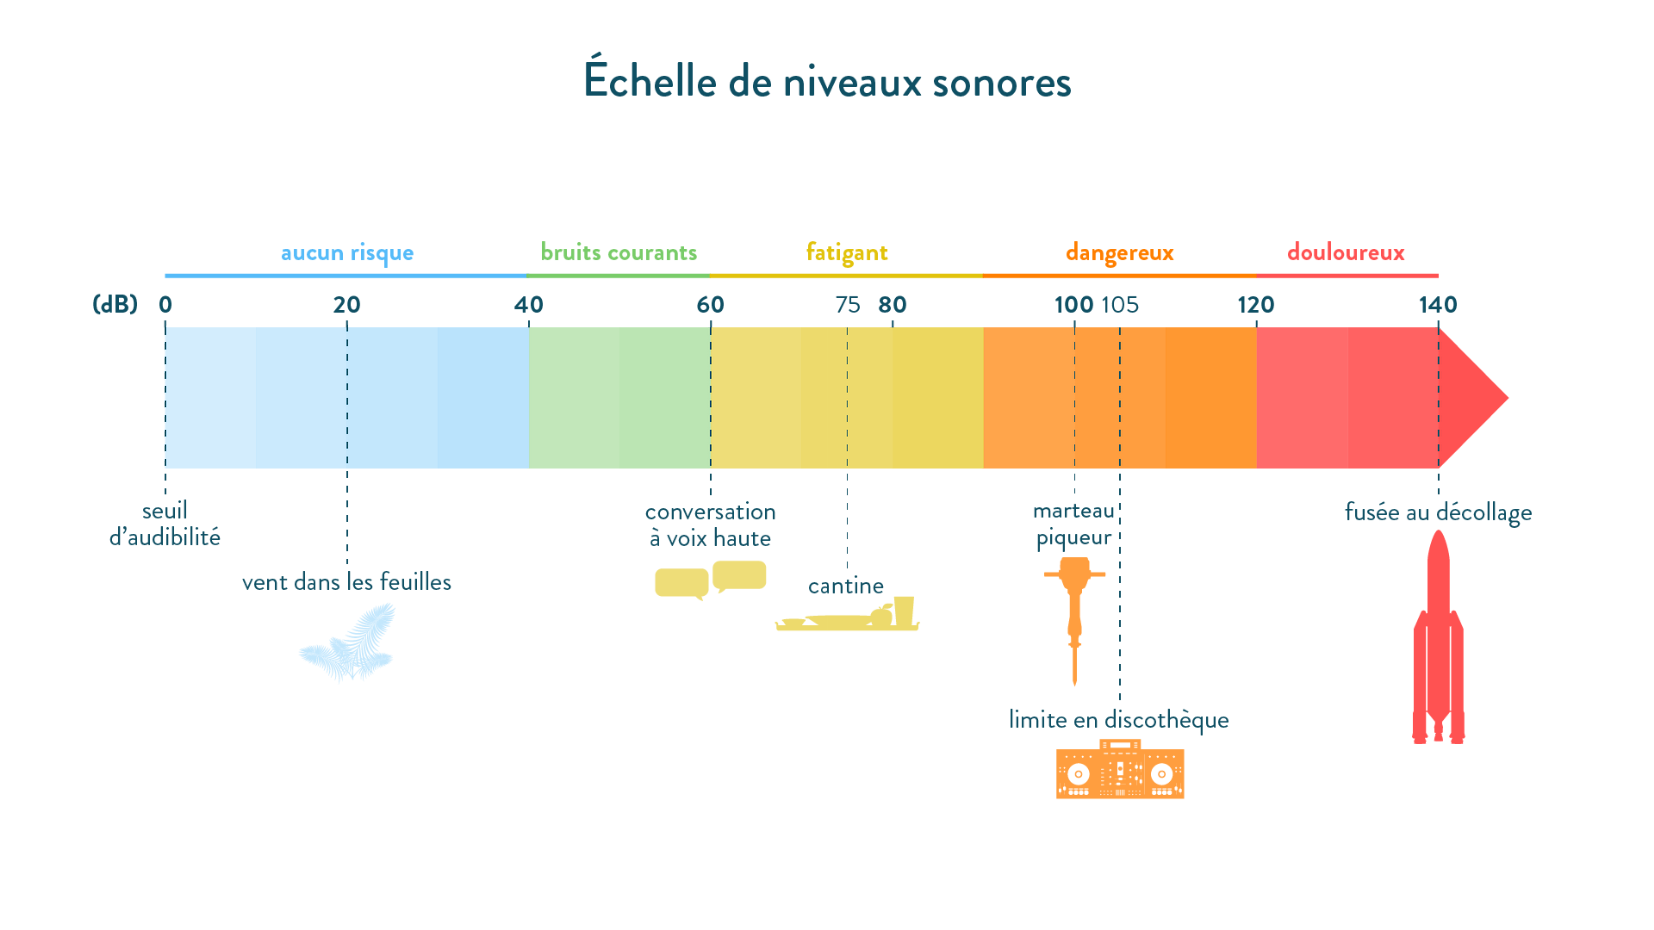
\includegraphics[scale=1.1]{images/dB.png} 
\end{center}

\ding{202} Calculer le niveau sonore $L$ lié à une intensité de $I=3 \times 10^{-5} W/m^2$. Arrondir le résultat à l'unité. \\

\cadreblanc{22}
\ding{203} En utilisant l'échelle de niveaux sonores, retrouver à quel environnement correspond ce niveau : \\

\cadreblanc{25}

\newpage

\textbf{Exercice 5 - QCM - conversions de longueurs} -
Entourer la ou les bonnes réponses\\
\begin{multicols}{3}
\begin{enumerate}
\item Combien de micromètres y a-t-il dans un décamètre ?
\begin{enumerate}
\item[a.] $10^4$
\item[b.] $10^5$
\item[c.] $10^6$
\item[d.] $10^7$
\item[e.] Aucune des réponses proposées
\end{enumerate}



\item Combien de micromètres y a-t-il dans un centimètre?
\begin{enumerate}
\item[a.] 10
\item[b.] 100
\item[c.]  1 000
\item[d.] 10 000 
\item[e.] Aucune des réponses proposées
\end{enumerate}






\item Combien de femtomètres y a-t-il dans un centimètre ?
\begin{enumerate}
\item[a.] $10^3$
\item[b.] $10^6$
\item[c.] $10^{13}$
\item[d.] $10^{15}$
\item[e.] Aucune des réponses proposées
\end{enumerate}

\item Combien de décamètres y a-t-il dans un millimètre ?
\begin{enumerate}
\item[a.] $10^{-6}$
\item[b.] $10^{-5}$
\item[c.] $10^{-4}$
\item[d.] $10^{-3}$
\item[e.] Aucune des réponses proposées
\end{enumerate}

\columnbreak



\item Combien de centimètres y a-t-il dans un décamètre ?
\begin{enumerate}
\item[a.] 1
\item[b.] 10
\item[c.] 100
\item[d.] 1000
\item[e.] Aucune des réponses proposées
\end{enumerate}




\item Combien de picomètres y a-t-il dans un millimètre ?
\begin{enumerate}
\item[a.] $10^{12}$
\item[b.] $10^{13}$
\item[c.] $10^{14}$
\item[d.] $10^{15}$
\item[e.] Aucune des réponses proposées
\end{enumerate}




\item Combien de centimètres y a-t-il dans un kilomètre ?
\begin{enumerate}
\item[a.] 1 000
\item[b.] 10 000
\item[c.] 100 000
\item[d.] 1 000 000
\item[e.] Aucune des réponses proposées
\end{enumerate}




\item Combien de picomètres y a-t-il dans un mètre ?
\begin{enumerate}
\item[a.] $10^{12}$
\item[b.] $10^{13}$
\item[c.] $10^{14}$
\item[d.] $10^{15}$
\item[e.] Aucune des réponses proposées
\end{enumerate}

\columnbreak


\item Combien de centimètres y a-t-il dans un hectomètre ?
\begin{enumerate}
\item[a.] 100
\item[b.] 1 000
\item[c.] 10 000
\item[d.] 100 000
\item[e.] Aucune des réponses proposées
\end{enumerate}
\item Combien de attomètres y a-t-il dans un kilomètre ?
\begin{enumerate}
\item[a.] $10^{12}$
\item[b.] $10^{15}$
\item[c.] $10^{18}$
\item[d.] $10^{21}$
\item[e.] Aucune des réponses proposées
\end{enumerate}
\end{enumerate}

\dotfill

Indications :

1 millimètre (mm) = $10^{-3}$ m

1 micromètre ($\mu$m) = $10^{-6}$ m

1 nanomètre (nm) = $10^{-9}$ m

1 picomètre (pm) = $10^{-12}$ m

1 femtomètre (fm) = $10^{-15}$ m

1 attomètre (am) = $10^{-18}$ m

1 kilomètre (km) = 1000 m

1 centimètre (cm) = 0.01 m

1 décimètre (dm) = 0.1 m

1 décamètre (dam) = 10 m

1 hectomètre (hm) = 100 m

\end{multicols}
\fbox{\textbf{BONUS +2 point }}\\[2mm]

Le son se déplace à une vitesse de 343 mètres par seconde dans l'air à une température de 20 C. Cependant, la vitesse du son varie en fonction de la température de l'air. Si la température de l'air augmente de 1 degré Celsius, la vitesse du son augmente de 0,6 mètres par seconde. Si la température de l'air baisse de 1 degré Celsius, la vitesse du son diminue de 0,6 mètres par seconde.\\
Si un avion vole à une altitude de 10 000 mètres, à quelle température de l'air la vitesse du son serait-elle la moitié de la vitesse de 340 mètres par seconde ?\\
\textbf{Indice} : Utilisez la formule de la vitesse du son en fonction de la température (v = 331 + 0,6 T, où v est la vitesse en mètres par seconde et T est la température en degrés Celsius).

\cadreblanc{10}

\end{document}